\documentclass{article}
\usepackage{ctex}          % 中文支持，适配中文排版
\usepackage{geometry}      % 页面布局设置
\usepackage{amsmath}       % 数学公式支持
\usepackage{amssymb}       % 数学符号支持
\usepackage{enumitem}      % 列表格式自定义
\usepackage{graphicx}      % 图片插入必备宏包
\usepackage{wrapfig}       % 图片环绕排版
\geometry{a4paper, margin=2.5cm} % A4纸，页边距2.5cm

% 设置图片路径
\graphicspath{{./}} 
% 图片缺失容错
\DeclareGraphicsExtensions{.jpg,.png,.pdf}
\DeclareGraphicsRule{*}{eps}{*}{}

\begin{document}
% 新题头（替换原\maketitle内容）
\begin{center}
    \Large\textbf{哈尔滨工业大学(深圳) 2025 学年春季学期} \\[0.5em]
    \Huge\textbf{电路IB合模拟电子技术基础 试 题（回忆版）} \\[1em]
    \normalsize
    注：本卷由 Slacker Deer 编写，纯靠记忆不涉及作弊行为，部分题目模糊、叙述有误等，恳请斧正。 \\[0.3em]
    本试卷考试时间 120 分钟，满分 100 分。 \\[1em]
    \large\textbf{注意行为规范 遵守考场纪律}
\end{center}

\vspace{1em} % 空一行

% 一、填空题
\section*{一、填空题（每题1分，共20分）}
\begin{enumerate}[label=\arabic*.]
    \item 引入电压负反馈的效果：\underline{\hspace{2em}}；引入串联负反馈的效果：\underline{\hspace{2em}}
    \item 已知$V_{cc}$，$R$，$R_{e0}$，$R_{e1}$，$\beta$且$\beta$远大于2，请问$I_{C1}$是\underline{\hspace{2em}}
      \begin{center}
          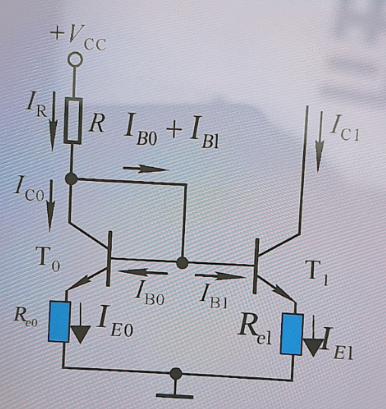
\includegraphics[width=0.7\textwidth]{2.jpg} 
          \vspace{0.3em} \\
      \end{center}
    \item 放大电路静态分析\underline{\hspace{2em}}（答案是静态工作点），两种分析方法：\underline{\hspace{2em}}、\underline{\hspace{2em}}
    \item PN结外加反向电压：\underline{\hspace{1.5em}} 抑制、\underline{\hspace{1.5em}} 加剧，\underline{\hspace{1.5em}}，\underline{\hspace{1.5em}}（注：后两空题目暂缺,书本上原话）
    \item $D_{Z1}$稳压电压为3$V$，$D_{Z2}$稳压电压为6$V$，请问$u_{o1}$：\underline{\hspace{2em}}，$u_{o2}$：\underline{\hspace{2em}}
      \begin{center}
          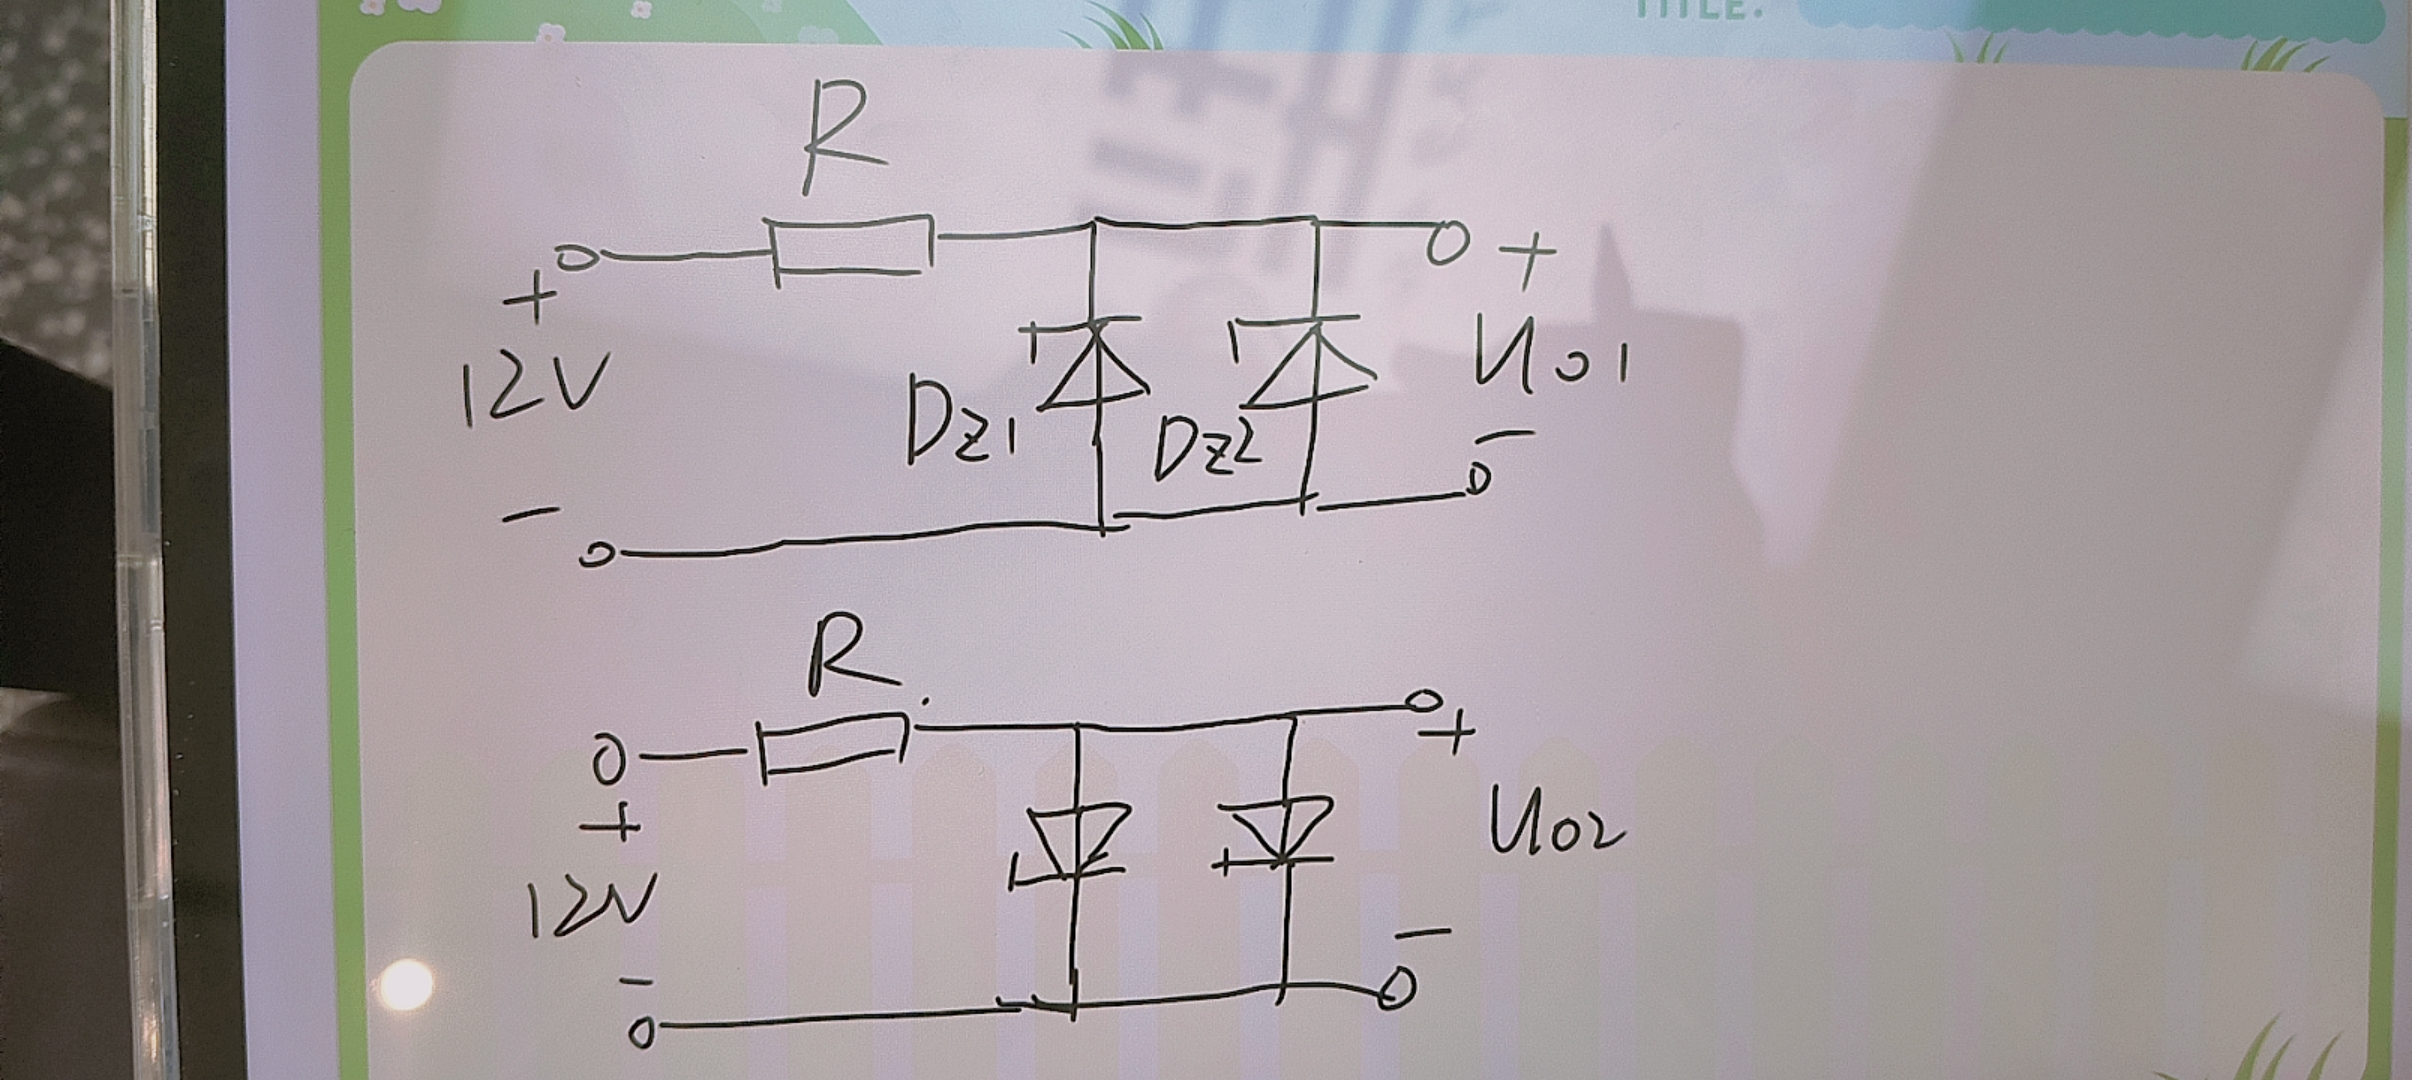
\includegraphics[width=0.7\textwidth]{5.jpg} 
          \vspace{0.3em} \\
      \end{center}
    \item 电路二端口中，若$\text{A}_\text{a}$、$\text{A}_\text{b}$分别为两个子二端口网络的传输参数矩阵，则复合二端口网络的传输参数矩阵$\text{A}_{\text{ab}}$与$\text{A}_\text{a}$、$\text{A}_\text{b}$的关系为：\underline{\hspace{4em}}
    \item 放大电路在低频区域的增益主要由\underline{\hspace{3em}}（填电路元件类型）决定
    \item 下图输出波形产生的失真为\underline{\hspace{2em}}，是由于放大电路晶体管工作在\underline{\hspace{2em}}区导致的。
      \begin{center}
          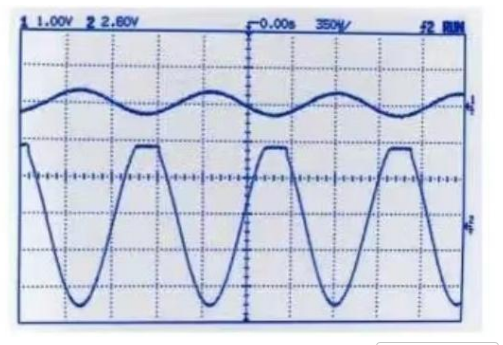
\includegraphics[width=0.7\textwidth]{8.jpg} 
          \vspace{0.3em} \\
          注：图中为输出波形的失真示意图
      \end{center}
    \item 形成驻波的两个条件：
          \begin{enumerate}[label=\arabic*.]
              \item \underline{\hspace{2em}}
              \item \underline{\hspace{2em}}
          \end{enumerate}
    \item 这是一段无损线，前一段Zc1为$60\Omega$，后一段Zc2为$100\Omega$,然后要使两个终端均不发生反射,问两个电阻分别是多少：\underline{\hspace{3em}}
    \begin{center}
        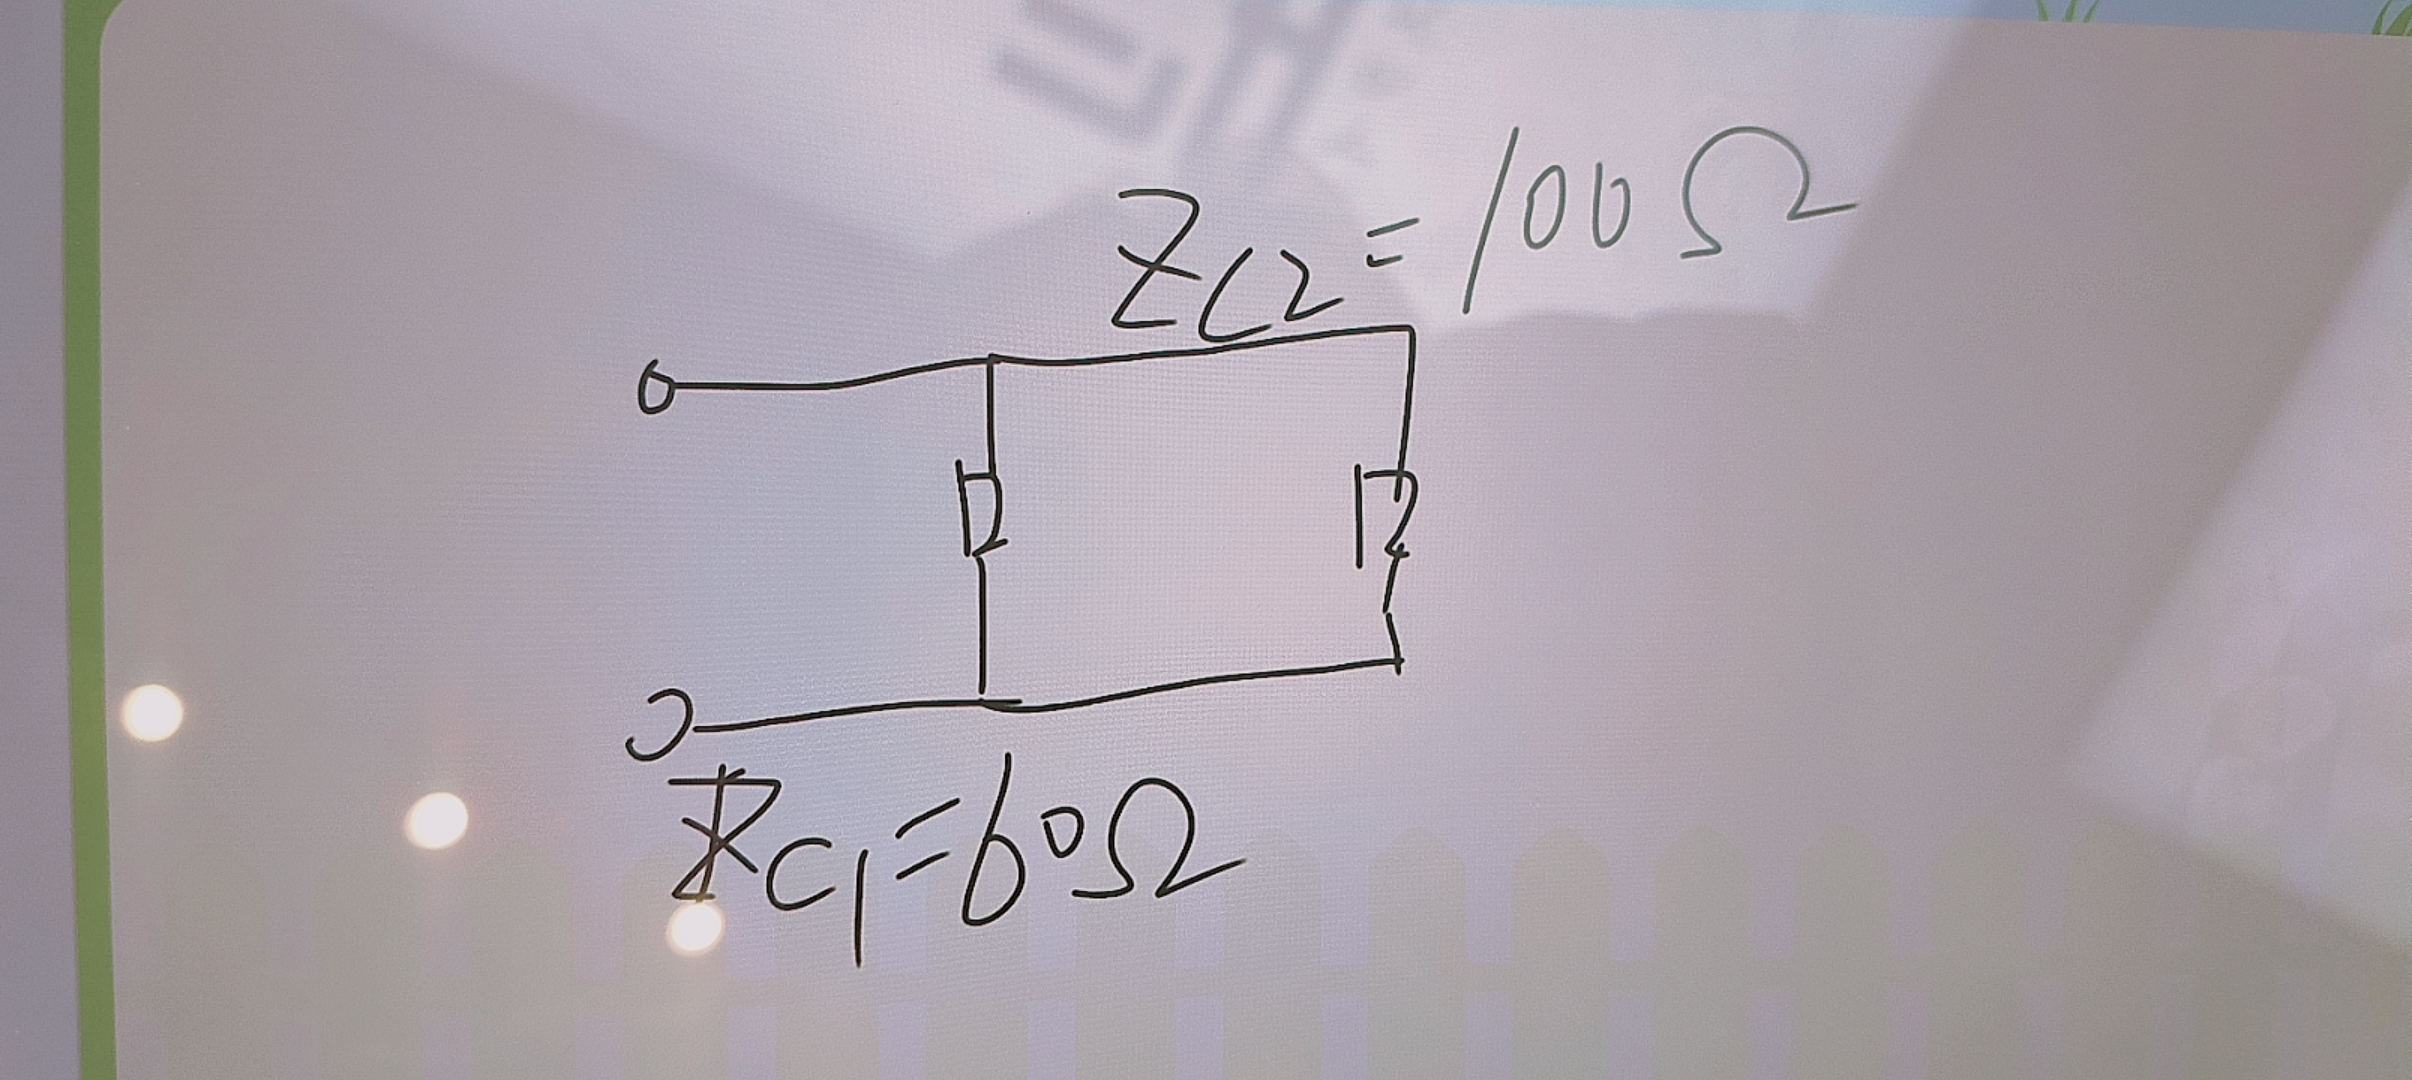
\includegraphics[width=0.8\textwidth]{10.jpg}
    \end{center}
\end{enumerate}

\vspace{1em}

% 二、简答题（分值按大题分配，共10分）
\section*{二、简答题（分值按大题分配，共10分）}
\begin{enumerate}[label=\arabic*.]
    \item （2.1）已知图示网络$\text{N}$的阻抗参数矩阵为 $\boxed{Z} = \begin{bmatrix} 5 & 4 \\ 4 & 5 \end{bmatrix}\ \Omega$，求复合二端口网络的传输参数矩阵。（原题给的是Y参数矩阵，并且不对称）
      \vspace{0.5em}
      \begin{center}
          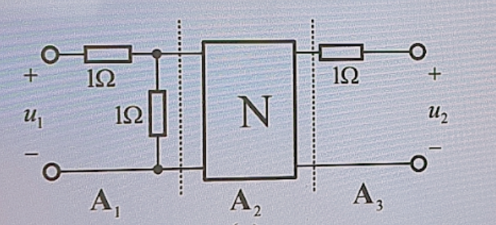
\includegraphics[width=0.6\textwidth]{二1.jpg} % 替换为你的图片文件名
      \end{center}
    \item 下边两个电路图是否能发生正弦振荡，能的说明理由，不能的说明理由并且给出如何修改这个电路使它能发生正弦振荡
      \begin{center}
          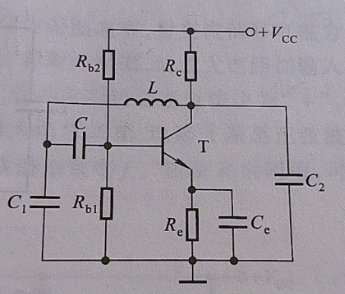
\includegraphics[width=0.6\textwidth]{二2_1.jpg} % 替换为你的图片文件名
          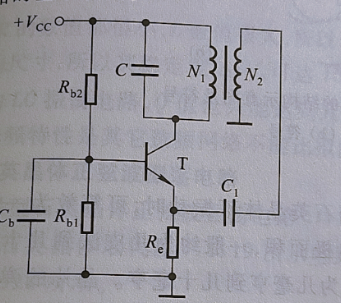
\includegraphics[width=0.6\textwidth]{二2_2.jpg} % 替换为你的图片文件名
      \end{center}
\end{enumerate}

\vspace{1em}

% 三、计算题
\section*{三、计算题（分值按大题分配，共10分/题）}
\begin{enumerate}[label=\arabic*., wide=0pt, leftmargin=*]
    \item 小信号分析：已知$U_S=2.4\ \text{V}$、$u_s(t)=0.28\cos \omega t$、$R=1\ \Omega$，$u = i + 0.4i^2$（均为串联）图中有两个电源串联
    \begin{center}
        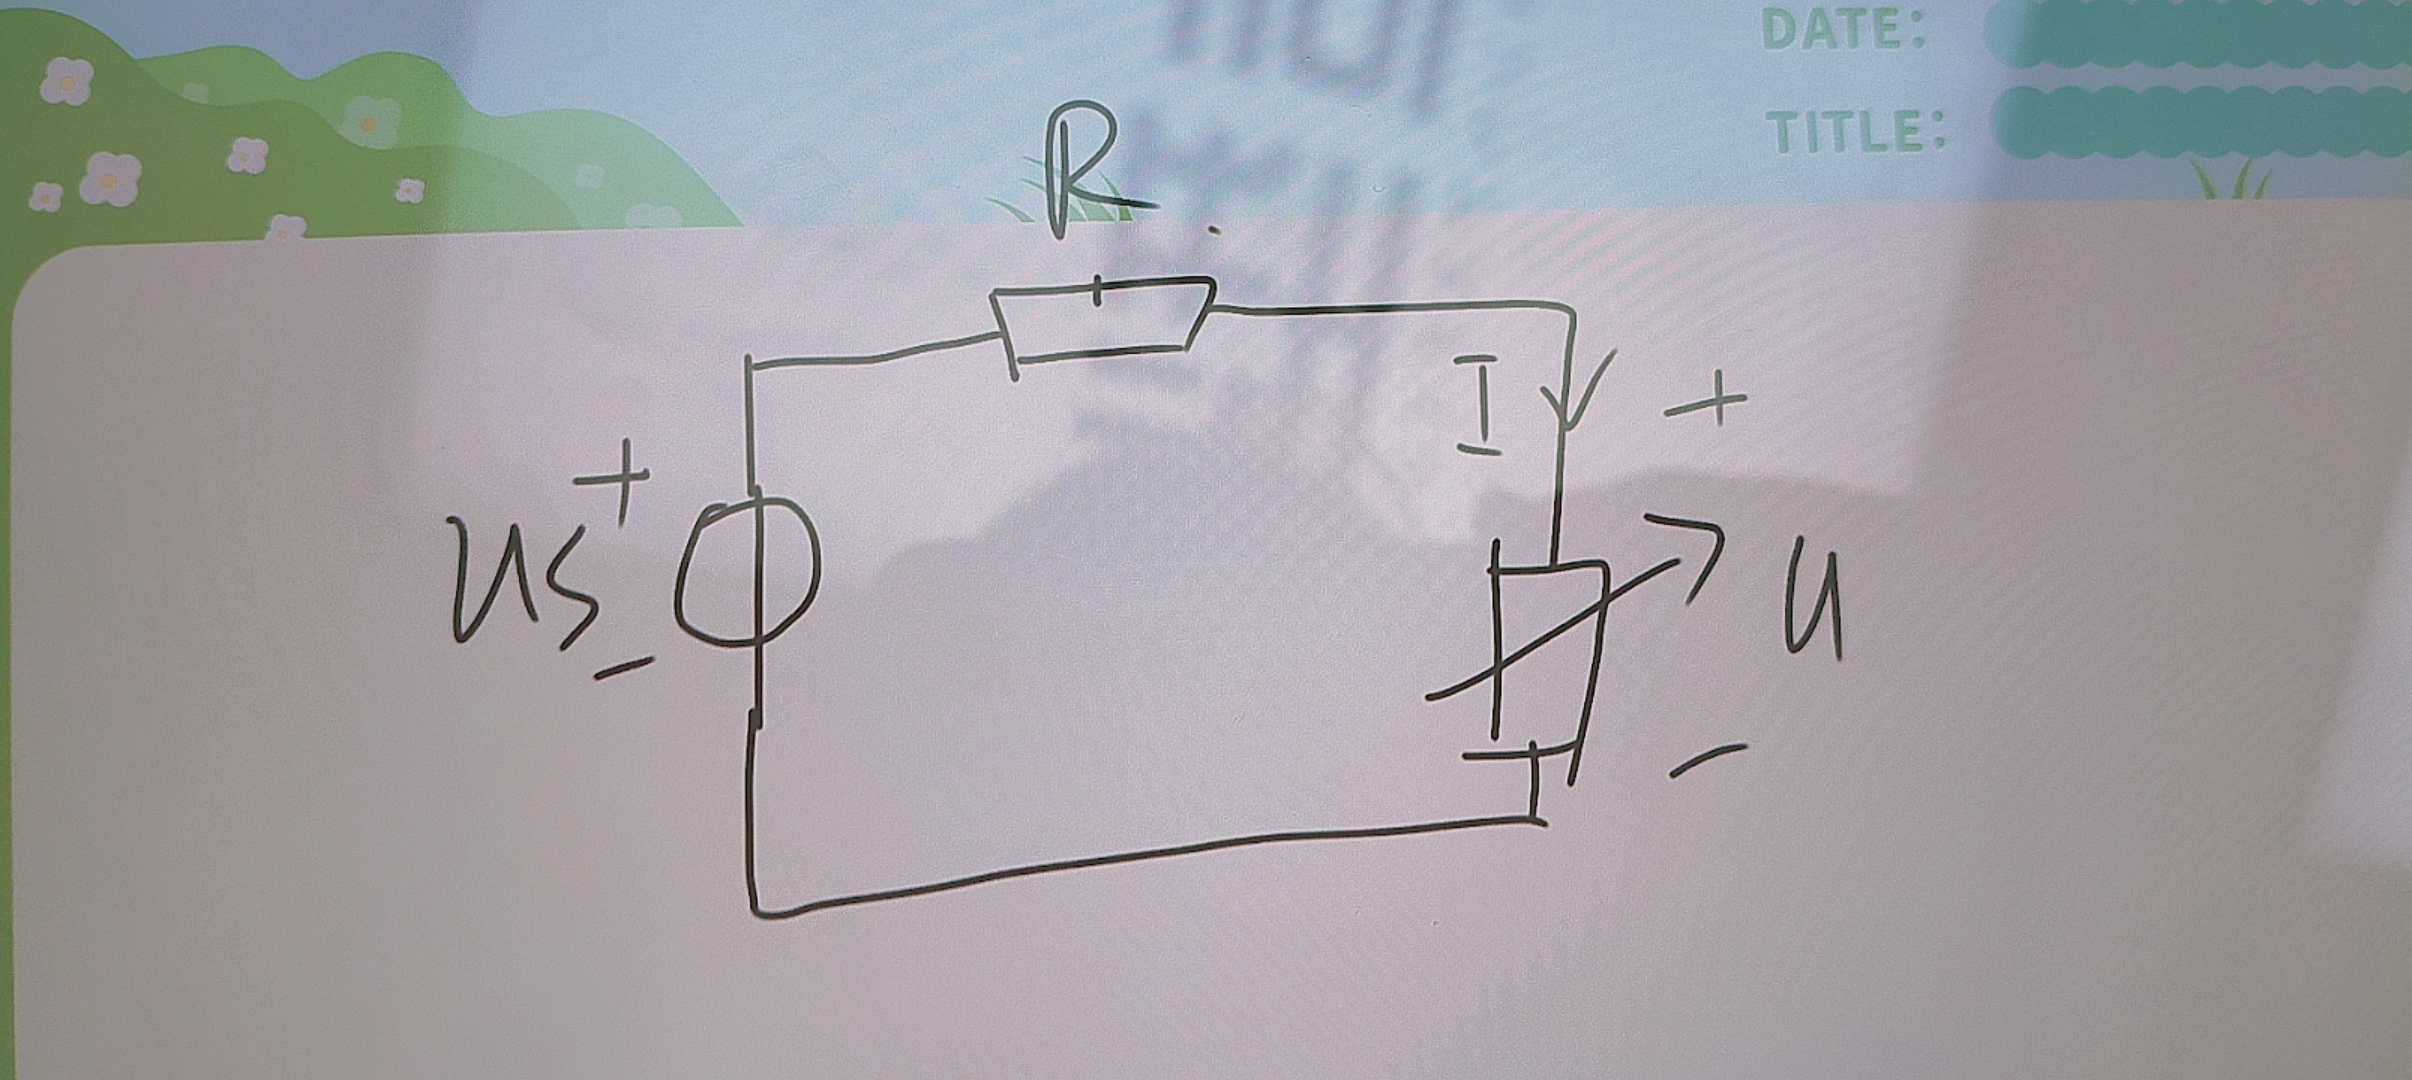
\includegraphics[width=0.8\textwidth]{三1.jpg}
    \end{center}
       \begin{enumerate}[label=(\arabic*)]
          \item 只有直流电源作用时，回路中的电流；
          \item 小信号作用时，小信号工作点的电压和电流；
      \end{enumerate}
    \item 预算放大器和稳压器构成的稳压电路如下，$R_1=R_4=3.3\text{k}\Omega$，$R_2=1.5\text{k}\Omega$，$v_i$两端并联一个电容
      \begin{enumerate}[label=(\arabic*)]
          \item 在下图中标注运算放大器的正负输入端；
          \item 求出输出电压$v_o$的可调节范围；
          \item 指出该电路存在的潜在问题。
      \end{enumerate}
    % 修正wrapfigure参数（原参数缺失，改为居中显示图片）
    \begin{center}
        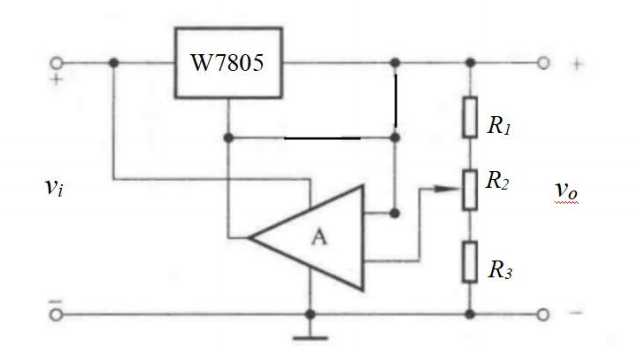
\includegraphics[width=0.8\textwidth]{三2.jpg}
    \end{center}
    \vspace{1em}
    
    \item 电路如下图所示：
      \begin{enumerate}[label=(\arabic*)]
          \item 写出 $u_{\text{o1}}$、$u_{\text{o2}}$ 与 $u_{\text{i}}$ 之间的关系表达式；
          \item 写出 $u_{\text{o}}$ 与 $u_{\text{o1}}$、$u_{\text{o2}}$ 和 $U_{\text{REF}}$ 之间的关系表达式。
      \end{enumerate}
      \vspace{0.5em}
      \begin{center}
          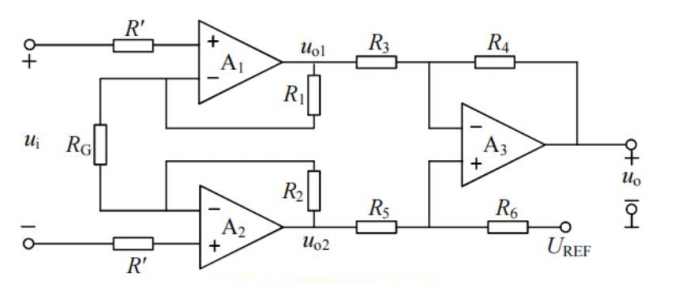
\includegraphics[width=0.8\textwidth]{三3.jpg} 
      \end{center}
    
    \item 功率放大电路如图所示，其中 $V_{\text{CC}}=15\text{V}$，$R_{\text{L}}=10\ \Omega$。试估算输出电压最大幅度 $U_{\text{omax}}$、输出功率最大值 $P_{\text{omax}}$、功率管 $\text{VT}_1$ 或 $\text{VT}_2$ 所承受的最大管压降 $U_{\text{CEMax}}$，电路会出现交越失真，如何调节电阻，请问A点的对地电压，A点为图中红点。
      \vspace{0.5em}
      \begin{center}
          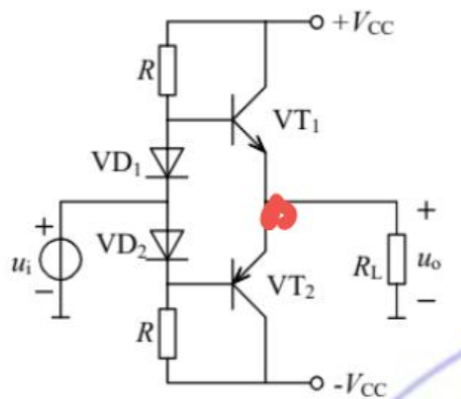
\includegraphics[width=0.7\textwidth]{三4.jpg} % 替换为你的图片文件名
          \vspace{0.3em} \\
      \end{center}
\end{enumerate}

\vspace{1em}

% 四、综合题（20分）
\section*{四、综合题（20分）}
\vspace{0.5em}
\begin{center}
    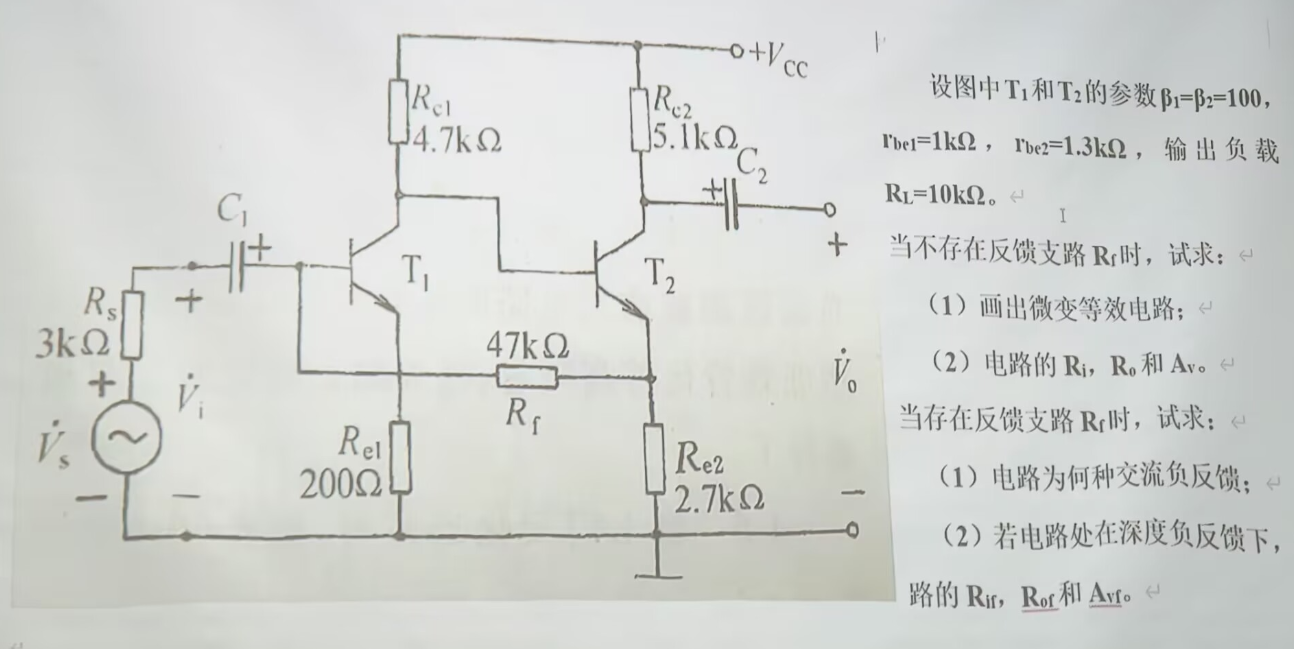
\includegraphics[width=0.8\textwidth]{四.jpg} 
\end{center}

\end{document}